\documentclass[11pt,a4paper]{article}
\usepackage[hyperref]{acl2020}
\usepackage{times}
\usepackage{latexsym}
\renewcommand{\UrlFont}{\ttfamily\small}
\usepackage{microtype}
\usepackage{amsmath}
\usepackage{changepage}
\usepackage[margin=1in,left=0.5in]{geometry} % 设置左边距更小
\usepackage{caption} % 引入caption宏包
\usepackage{graphicx} % 导入插入图片的宏包
\usepackage{listings}
\usepackage{cite}
\usepackage{booktabs}
\usepackage{multirow}
\usepackage{cite}

\newcommand\BibTeX{B\textsc{ib}\TeX}

\title{Evaluating Impact of Social Media Posts 
on Stock Prices
}

\author{First Author \\
  Affiliation / Address line 1 \\
  Affiliation / Address line 2 \\
  Affiliation / Address line 3 \\
  \texttt{email@domain} \\\And
  Second Author \\
  Affiliation / Address line 1 \\
  Affiliation / Address line 2 \\
  Affiliation / Address line 3 \\
  \texttt{email@domain} \\}

\date{}

\begin{document}
\maketitle
\begin{abstract}
  This study explores the influence of social media sentiment on stock market behavior using Apple Inc. (AAPL) . A dataset comprising 1.4 million tweets spanning from 2015 to 2020, along with AAPL's historical trading data, was analyzed to uncover sentiment-driven market insights. The research unfolds across three distinct experiments: The first validates the impact of social media commentary on stock prices, confirming that public sentiment correlates with market movements. The second experiment involves a comparative analysis of various neural network architectures, including RNN, LSTM, GRU, and MLP, to identify the most effective model for our dataset, which was found to be the MLP. The third experiment employs the MLP model in a simulated quantitative trading scenario to assess the practical applicability of sentiment-driven trading strategies. By integrating sentiment analysis tools like VADER and FinBERT with stock market data, this study not only corroborates the significance of social media sentiment in predicting stock prices but also advances a data-driven trading approach, laying groundwork for future enhancements in both the methodology and application of sentiment analysis in finance.
\end{abstract}


\section{Introduction}

The intersection of finance and technology has seen revolutionary changes with the advent of machine learning and big data analytics. Among the most intriguing developments is the exploration of social media sentiment as a potential indicator of stock market movements. The rationale behind this interest lies in the hypothesis that the collective mood and opinions expressed on social media platforms can influence, or at least predict, the fluctuations in stock prices. This study aims to delve into this premise by examining the relationship between social media sentiment and the stock prices of Apple Inc. (AAPL), a leading company in the technology sector with a significant presence in both the market and media.Apple Inc. was chosen as the  representative for this study due to its high profile and significant market capitalization, which ensures a consistent and substantial volume of discourse on social media platforms. Furthermore, AAPL's broad consumer base and impact on global technology trends mean that its stock price is particularly sensitive to public sentiment, providing a robust case for analyzing the correlation between social media mood and market performance.


The surge of user-generated content on platforms such as Twitter has provided an abundance of data that reflects public perception in real-time. Unlike traditional financial indicators, which are grounded in numerical and often historical data, sentiment analysis offers a more nuanced and immediate gauge of public opinion and market sentiment. This research leverages sentiment analysis to quantify the emotional content in tweets related to AAPL over a period from 2015 to 2020, a timeframe that promises a rich dataset due to Apple company's continued innovation and market influence.

 this investigation is  structured in a threefold experimental design,first confirms the anticipated impact of social media commentary on stock prices, establishing a foundational link between sentiment and market behavior. The second phase rigorously scrutinizes a suite of neural network models to discern the optimal architecture for harnessing these insights.  The third and final experiment transitions from theory to application, deploying  model within a simulated quantitative trading framework to evaluate the feasibility of a sentiment-based trading strategy.

Previous studies have established a correlation between news sentiment and stock market performance. However, social media presents a novel and less structured data source that poses both opportunities and challenges. The spontaneous and conversational nature of Twitter, for instance, requires robust natural language processing (NLP) tools to accurately capture sentiment. To address this, our first experiment employs advanced sentiment analysis algorithms, namely VADER (Valence Aware Dictionary and sEntiment Reasoner) and FinBERT (a BERT-based model fine-tuned for financial text), to process and analyze the collected tweets,assigning sentiment scores to gauge the mood surrounding AAPL. These sentiment scores are then integrated into a simple LSTM model, serving as our baseline. We experiment with augmenting this baseline model by separately incorporating the sentiment scores obtained from VADER and FinBERT. The results of this integrative approach reveal a notable enhancement in the predictive accuracy of stock prices, with the incorporation of FinBERT sentiment scores proving to be more effective.

In the second phase of our study, we shift our focus to a comparative analysis of various neural network architectures, delving into how each model—RNN, GRU, LSTM, and MLP—performs in the context of stock price prediction. This experiment entails using each of these models as a baseline and then integrating the FinBERT sentiment scores to assess their impact on the predictive capabilities. The models are evaluated both before and after the inclusion of these sentiment scores, providing a clear picture of how the addition of sentiment analysis influences the accuracy of stock price predictions. Through this comparative process, the MLP model emerges as the most effective, demonstrating ability to incorporate FinBERT-derived sentiment data for enhanced stock market forecasting.

The third experiment employs the MLP model in a simulated quantitative trading scenario to assess the practical applicability of sentiment-driven trading strategies



\section{Related Work}
\subsection{VADER}
VADER \cite{roehrick2020valence} is a rule-based sentiment analysis tool designed for social media texts. It uses lexical and grammatical heuristics to determine sentiment. It has a sentiment lexicon with word scores and considers linguistic features to gauge sentiment intensity. VADER handles negation words and is effective for sentiment analysis in informal text. However, it may struggle with sarcasm, irony, or complex language.
\subsection{FinBERT}
FinBERT \cite{araci2019finbert} is a specialized language model for financial sentiment analysis. It incorporates financial domain-specific knowledge and is trained on financial text, including news articles and social media posts. It can accurately analyze sentiment in the financial domain by capturing contextual features and financial jargon. FinBERT has shown impressive performance in various financial sentiment analysis tasks. However, its effectiveness may be limited outside the financial domain or with non-finance-related text.
\subsection{BERT}
BERT \cite{devlin2018bert} is a powerful language model introduced by Google in 2018. It revolutionized natural language processing (NLP) by capturing contextual information and achieving state-of-the-art performance. BERT is pre-trained on diverse text sources and learns contextual understanding through masked language modeling and next sentence prediction. Its bidirectional nature allows it to effectively capture and utilize contextual information. BERT can be fine-tuned for specific NLP tasks and has been widely used in text classification, named entity recognition, question answering, and sentiment analysis. While BERT has limitations such as computational cost and long-range dependency handling, it has had a significant impact on NLP and paved the way for subsequent models and techniques.
\subsection{RNNs}
Recurrent Neural Networks (RNNs) are neural network architectures designed for sequential data processing. They can capture information from previous steps in a sequence, making them suitable for tasks like natural language processing, speech recognition, and time series analysis. RNNs maintain a hidden state that retains information about the sequence. Traditional RNNs face the vanishing gradient problem, but variants like LSTM and GRU have gating mechanisms to address this issue. RNNs have been applied in various domains, including language modeling, sentiment analysis, machine translation, speech recognition, and time series analysis. However, RNNs can be computationally expensive and may struggle with very long sequences. Despite these limitations, RNNs remain a fundamental architecture in deep learning for sequential data tasks.
\subsubsection{LSTM}
Long Short-Term Memory (LSTM) is a specialized variant of Recurrent Neural Networks (RNNs) designed to address the vanishing gradient problem and capture long-term dependencies in sequential data. LSTMs use gates to selectively retain, forget, and expose information over time. The introduction of a memory cell allows LSTMs to maintain and update information, enabling them to capture complex sequential patterns. LSTMs have been successfully applied in various domains, including natural language processing, speech recognition, machine translation, and time series analysis. They excel in tasks involving long-range dependencies. However, LSTMs can be computationally expensive and require substantial training data. Designing and tuning LSTM architectures can be challenging, and overfitting remains a concern. Nonetheless, LSTMs are widely used and an integral part of many cutting-edge deep learning models for sequential data processing.
\subsubsection{GRU}
Gated Recurrent Unit (GRU) is a type of recurrent neural network (RNN) that addresses the vanishing gradient problem and captures long-term dependencies in sequential data. GRUs have gained popularity as a simpler alternative to traditional RNNs and have been widely used in various sequential data processing tasks.
Similar to LSTMs, GRUs incorporate gating mechanisms to control the flow of information. However, GRUs have a simpler architecture with fewer gating components. They employ two main gates: the update gate and the reset gate. The update gate determines the amount of information to be updated and stored, while the reset gate controls the influence of past information on the current state. These gates allow GRUs to selectively update and forget information, enabling them to capture long-term dependencies efficiently.
GRUs have been applied successfully in tasks such as natural language processing, speech recognition, recommendation systems, and video analysis. They offer advantages such as simpler architecture, faster training convergence, and lower memory requirements compared to traditional RNNs. GRUs have demonstrated competitive performance and computational efficiency, making them suitable for applications with limited computational resources.
However, the choice between GRUs and LSTMs depends on the specific task and dataset. Empirical evaluation is necessary to determine the most appropriate architecture. Overall, GRUs are a valuable subclass of RNNs that effectively capture long-term dependencies in sequential data, providing an alternative to LSTMs with competitive performance.
\subsubsection{Bidirectional RNNs}
Bidirectional Recurrent Neural Networks (RNNs)\cite{schuster1997bidirectional} capture both past and future contextual information in sequential data by processing the input sequence in both forward and backward directions. They have shown improvements in tasks involving sequential data and are particularly effective when current elements depend on both past and future elements. However, they require the entire sequence upfront and can be computationally expensive.
\subsection{MLP}
The Multilayer Perceptron (MLP) is a widely used type of artificial neural network. It consists of multiple layers of interconnected neurons, including an input layer, one or more hidden layers, and an output layer. MLPs can learn complex relationships in data by using activation functions and adjusting weights through backpropagation. They have been applied to various tasks but may struggle with high-dimensional data and overfitting. Other advanced neural network architectures, like CNNs and RNNs, have gained popularity in certain domains. In summary, the Multilayer Perceptron (MLP) is a versatile and widely used neural network architecture that can capture complex patterns in data. While newer architectures have emerged, MLPs remain a fundamental approach in machine learning and serve as a foundation for more advanced deep learning techniques.



\section{Data}
\subsection{Data Collection}
This research utilizes two primary datasets to explore the relationship between social media sentiment and stock prices.

\subsubsection{Twitter Data}
The first dataset consists of Twitter posts, specifically targeting mentions of Apple Inc. (AAPL). A total of 1,424,714 tweets from the period of 2015 to 2020 were collected, providing a comprehensive view of public sentiment during this time. Each tweet includes several features: the posting date, the username of the author, and the body of the tweet. This data was sourced from the publicly available Kaggle dataset, which can be found at \url{https://www.kaggle.com/datasets/omermetinn/tweets-about-the-top-companies-from-2015-to}
\url{-2020}.

\subsubsection{Historical Stock Data}
The second dataset encompasses historical trading data for AAPL, totaling 1,258 trading days between 2015 and 2020. This dataset includes the opening price ('open'), the highest price of the day ('high'), the lowest price ('low'), the total trading volume ('volume'), and the closing price ('close') of AAPL stock for each trading day. The data was retrieved from Yahoo Finance, which is a reputable source for such financial information.
\subsection{Data Preprocessing}
Data preprocessing is a critical step in any data analysis process as it ensures data quality and prepares the input for effective model training.

\subsubsection{Sentiment Analysis Preprocessing}
The sentiment analysis involved processing the collected tweets to quantify the sentiment expressed towards Apple Inc. (AAPL). We utilized two sentiment analysis tools, VADER and FinBERT, to assign sentiment scores to the tweets. VADER, designed for social media text, provides scores across a spectrum from negative to positive. FinBERT, a BERT-based model fine-tuned for financial contexts, offers a more nuanced sentiment classification, tailored to the financial domain. The output from these tools includes a sentiment score and a label categorizing the sentiment as positive, negative, or neutral. These scores and labels are essential features for the subsequent predictive modeling.

\subsubsection{Stock Data Preprocessing}
Stock data preprocessing included the removal of outliers and normalization of price data to adjust for any stock splits or dividends. We conducted outlier detection on the opening, high, low, and closing prices using box plots to ensure that extreme values, which could be due to market anomalies or data collection errors, do not skew the analysis. This step helped in identifying and handling anomalous fluctuations in stock prices that could affect the model's performance.


\subsubsection{Feature Extraction}
We introduced new variables such as the exponentially weighted moving average (EWMA) of the closing prices over different time spans (3, 7, 14, and 30 days). These variables capture both short-term and long-term trends in the stock prices, providing our models with the ability to detect patterns over multiple time horizons.


\subsubsection{Feature Selection}
Feature selection involved aggregating sentiment scores on a daily basis and merging them with the stock data. Each day's sentiment was represented as an average of the scores from all tweets posted on that day. This merged dataset, now enriched with both sentiment and stock data, underwent a feature selection process to retain only the most informative features. After dropping around 100 less significant data points, the final dataset consisted of the selected features ready to be used as inputs (X) and outputs (Y) for model training.

\subsection{Merged Dataset }

The merged dataset prepared for modeling contained the following attributes:finbert sentiment scores (neutral, positive, negative), and the compound VADER score; the number of comments per tweet (comment\_num), and key stock price indicators (open, high, low, close, volume). Additionally, the dataset included exponentially weighted moving averages (EWMAs) for various periods((3, 7, 14,
and 30 days), capturing both short-term and long-term price movements.



\subsubsection{Training, Test, and Validation Dataset Splitting}

The dataset is partitioned into three distinct subsets: training, validation (development), and testing sets. This segmentation facilitates the various phases of model development and evaluation. The partitioning is done as follows:


\begin{itemize}
    \item \textbf{Training Set:} This subset constitutes 70\% of the data. It is used to train the model, allowing it to learn from this data.
    \item \textbf{Validation Set:} Comprising 15\% of the data, this set is utilized for tuning model parameters and for preliminary performance evaluation. This step is crucial for preventing overfitting and underfitting.
    \item \textbf{Testing Set:} The remaining 15\% of the data serves as the testing set. This set is used strictly for evaluating the model's performance after the training process. It provides an unbiased assessment of the model's effectiveness in handling new, unseen data

\end{itemize}



\section{Experiments and results}

    \subsection{Experiment 1: Validation of Sentiment Scores}

    This experiment aims to validate the effectiveness of sentiment scores derived from Twitter data in predicting the stock prices of Apple Inc. (AAPL). The analysis is based on a simple LSTM model that incorporates sentiment scores as features.
    
    \subsubsection{Model Description}
    The LSTM model was developed with the following input features:
    \begin{itemize}
        \item Stock data: Open, high, low, close prices, and volume.
        \item Sentiment scores: FinBERT and VADER sentiment scores, combined with a 4-point exponentially weighted moving average (EWMA) of the closing prices.
    \end{itemize}
    
    \subsubsection{Results}
    The performance of the LSTM model was evaluated using the following metrics: Mean Squared Error (MSE), Mean Absolute Error (MAE), and the R-squared (R2) value. The results are summarized in Table 1.
    
    \begin{table}[ht] % 使用[H]来精确放置表格
      \centering
      \caption{Summary of Model Performance Metrics}
      \label{tab:experiment1_results}
      \begin{tabular}{lccc}
      \toprule
      Model & MSE & MAE & R2 \\
      \midrule
      Base LSTM & 0.7849 & 0.6306 & -0.1772 \\
      LSTM with VADER & 0.7370 & 0.5891 & -0.1055 \\
      LSTM with FinBERT & 0.4846 & 0.5111 & 0.2731 \\
      \bottomrule
      \end{tabular}
      \end{table}
      
          
    From the table,the LSTM model utilizing FinBERT sentiment
    scores outperformed the base model and the one
    using Vader scores in terms of MSE and R2,
    indicating a better fit to the actual stock prices.    



    \subsubsection{Visual Representation}
    Figure 1 illustrates the comparison between the actual closing prices and the predictions made by the base LSTM model, as well as the models augmented with VADER and FinBERT sentiment scores.
    
    % Include the figure in your document by using the appropriate path to your image file
    \begin{figure}[ht]
    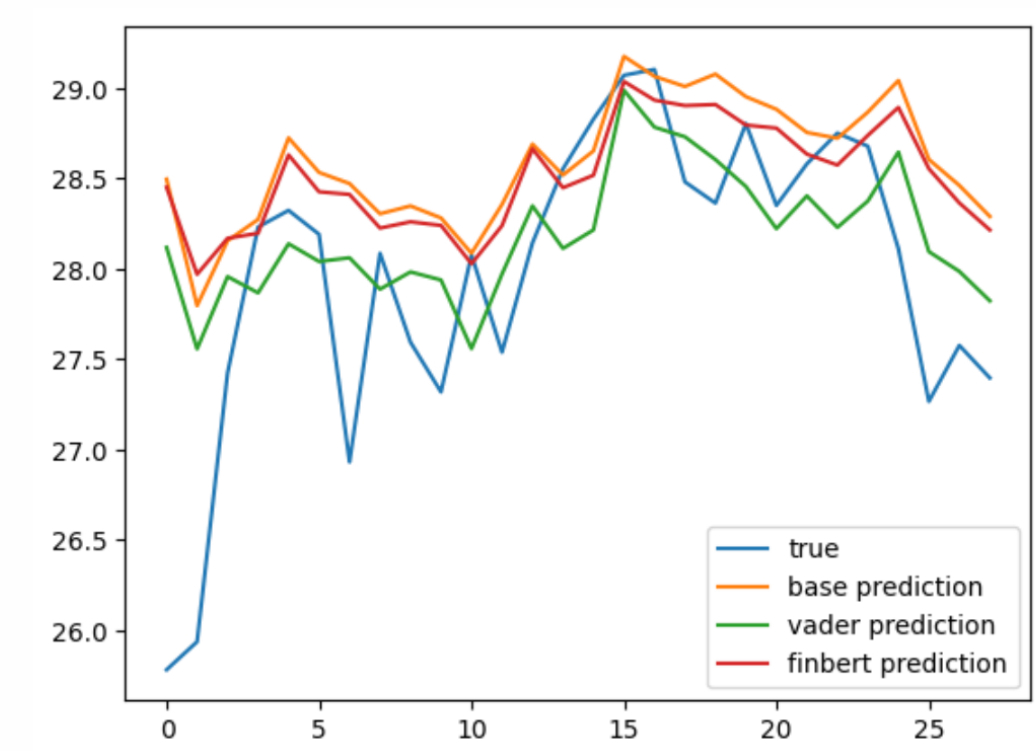
\includegraphics[width=0.5\textwidth]{figs/2023-11-29_220912.jpg}
    \caption{Comparison of Actual and Predicted AAPL Closing Prices}
    \label{fig:sentiment_validation}
    \end{figure}
    
    The graphical analysis indicates that the predictions incorporating sentiment scores, particularly those from finbert, align more closely with the actual stock price trends.
    

    \subsubsection{Conclusion}
    1.Social media sentiment has an impact on stock closing prices//
    2.The prediction effect of sentiment analysis made with FinBERT is the best, and subsequent experiments are based on this data set base + FinBERT



  \subsection{Experiment 2: Neural Network Model Comparison}
  \label{sec:experiment2}
  
  This experiment aims to compare different neural network architectures to determine the most effective model for predicting AAPL stock prices based on the sentiment scores and historical trading data.
  
  \subsubsection{Model Architectures}
  We evaluated four different types of neural network architectures: Recurrent Neural Network (RNN), Long Short-Term Memory (LSTM), Gated Recurrent Unit (GRU), and Multi-Layer Perceptron (MLP). Each model was first trained using historical stock data as the baseline. Then, we integrated the FinBERT sentiment scores to investigate the improvement in prediction accuracy.
  
  \subsubsection{Training and Evaluation}
  Each model was trained over 60 epochs with a batch size of 32. The performance was evaluated using the loss function, specifically the Mean Squared Error (MSE), which measures the average squared difference between the estimated values and the actual value.
  
  \subsubsection{Results}
  Figure 2 shows the loss of each model over the training epochs. It is evident from the graph that the MLP model converges to a lower loss value faster than the other models, suggesting a better predictive performance.
  
  \begin{figure}[ht]
  \centering
  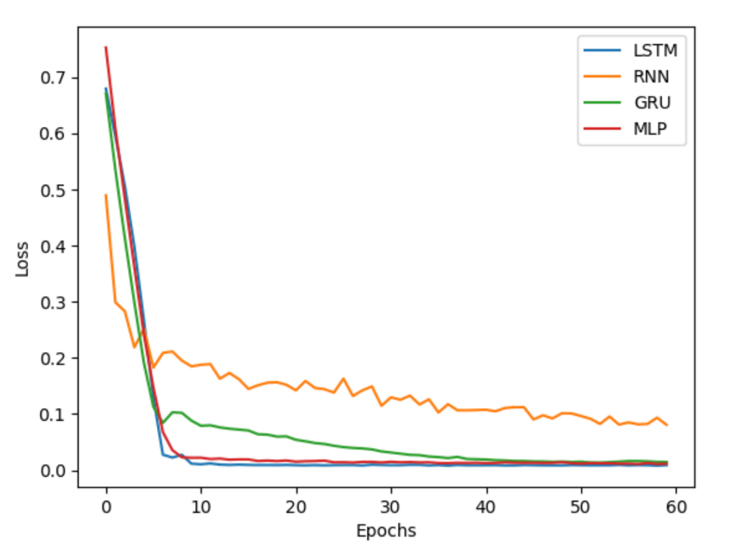
\includegraphics[width=0.5\textwidth]{figs/2023-11-29_230313.jpg}
  \caption{Loss of Different Models in Experiment 2}
  \label{fig:loss_comparison}
  \end{figure}
  
  We also compared the predicted stock prices with the actual values, as illustrated in Figure 3. The MLP model closely follows the true stock prices, indicating its superior predictive capability among the tested architectures.
  
  \begin{figure}[ht]
  \centering
  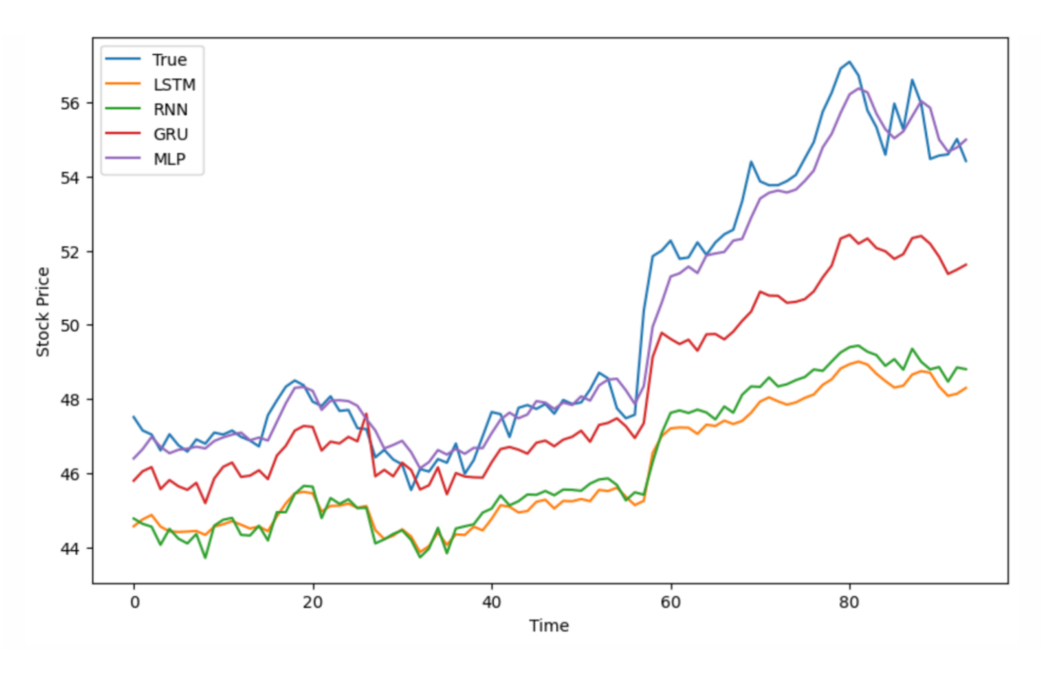
\includegraphics[width=0.5\textwidth]{figs/2023-11-30_161316.jpg}
  \caption{Comparison of Predicted and True AAPL Stock Prices}
  \label{fig:prediction_comparison}
  \end{figure}
  
  Figure 4 presents the Mean Absolute Error (MAE), Mean Squared Error (MSE), and R-squared (R2) metrics for each model on the validation set. The MLP model exhibits the lowest error metrics, confirming its effectiveness in the context of stock price prediction.
  
  \begin{figure}[ht]
  \centering
  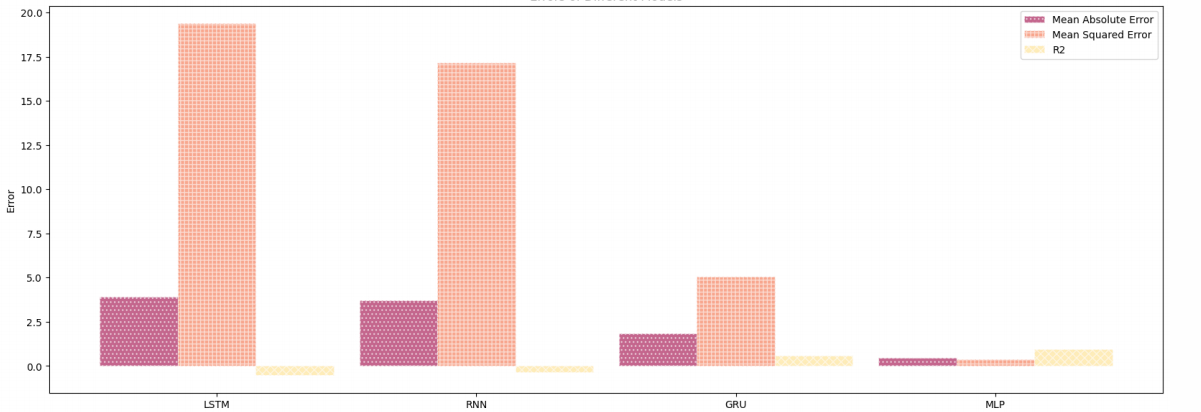
\includegraphics[width=0.5\textwidth]{figs/2023-11-29_230902.jpg}
  \caption{Error Metrics of Different Models}
  \label{fig:error_comparison}
  \end{figure}
  
  \subsubsection{Conclusion}
  The comparative analysis clearly demonstrates that the MLP model outperforms RNN, LSTM, and GRU in predicting stock prices when using the sentiment scores derived from FinBERT. Hence, the MLP model was chosen for further experimentation in the quantitative trading scenario.
  















  \subsection{Experiment 3: Quantitative Trading Strategy Simulation}
  \label{sec:experiment3}
  
  This experiment aims to evaluate the practical applicability of sentiment-driven trading strategies using the MLP model trained with FinBERT sentiment scores.
  
  \subsubsection{Trading Strategy}
  The trading strategy was devised based on the predictions made by the MLP model. A simple rule was followed: if the predicted closing price for the next day {close\_predict(t+1)} was higher than the actual closing price of the current day close\_actual(t), a long position was taken. Conversely, if the predicted closing price was lower than the actual closing price, the position was closed, assuming a short-selling scenario was not possible.
  
  \subsubsection{Simulation Results}
  The simulation results demonstrate the feasibility of a sentiment-based trading strategy. Figure 5 shows a comparison between the MLP model's predicted stock prices and the actual stock prices. 
  
  \begin{figure}[ht]
  \centering
  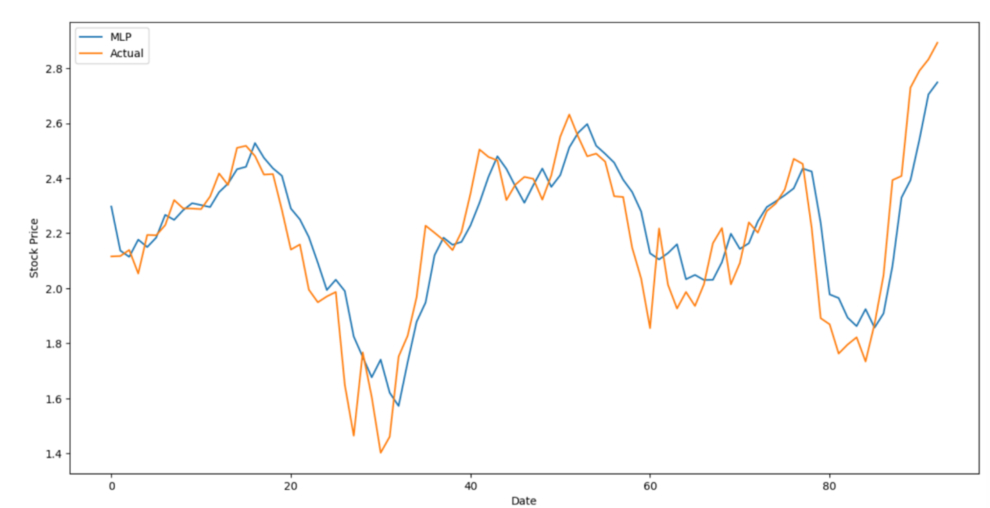
\includegraphics[width=0.4\textwidth]{figs/2023-11-30_143814.jpg}
  \caption{Comparison of MLP Predicted Stock Prices vs. Actual Prices}
  \label{fig:mlp_vs_actual_prices}
  \end{figure}
  
  Additionally, Figure 6 illustrates the investment value over time when applying the trading strategy based on the MLP model's predictions.
  
  \begin{figure}[ht]
  \centering
  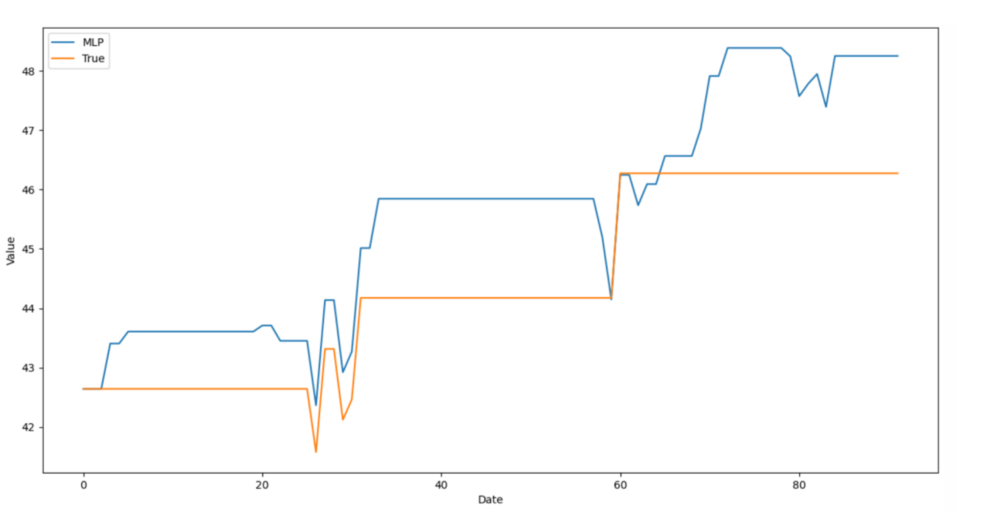
\includegraphics[width=0.5\textwidth]{figs/2023-11-30_143820.jpg}
  \caption{Investment Value Over Time Using MLP-Based Trading Strategy}
  \label{fig:trading_strategy_results}
  \end{figure}
  
  \subsubsection{Conclusion}
  The MLP model, when combined with FinBERT sentiment analysis, shows promise in simulating a trading strategy that outperforms a simple buy-and-hold strategy, as seen in the growth of investment value over time. This suggests that incorporating sentiment analysis into stock price prediction models can potentially yield profitable trading strategies.
  
  

















  \section{Limitations}

  This research encountered several technical and data-related challenges that impacted the study's scope and outcomes:
  
  \begin{itemize}
    \item \textbf{FinBERT API Limitations}: Encountered issues included an unstable API connection and an inability to process overly long texts, which could lead to incomplete sentiment analysis. Additionally, the computational time for processing was significant, indicating a need for more efficient sentiment analysis techniques.
    
    \item \textbf{Data Collection Constraints}: The time interval for data collection was constrained by the limits of the available Twitter dataset, leading to potential gaps in sentiment tracking. Moreover, null values introduced by the FinBERT API necessitated additional preprocessing steps which could affect the integrity of the sentiment analysis.
  \end{itemize}
  
  These limitations highlight the need for improved data handling and analysis frameworks to ensure robust and reliable sentiment analysis for stock price prediction.
  



  \section{Future Work}

  Building on the findings and limitations of this study, several avenues for future research have been identified:
  
  \begin{itemize}
    \item \textbf{Enhancing Model Resilience}: Future models should be designed to handle the missing values caused by server disconnection or API instability, ensuring continuous data analysis without loss of information.
    
    \item \textbf{Comparative Analysis}: A comparative study of the effects of social media comments from the general public versus corporate executives on stock price predictions would provide deeper insights into the different forces shaping market sentiment.
    
    \item \textbf{Quantitative Strategy Research}: There is a need to further explore quantitative trading strategies that incorporate sentiment analysis, potentially leading to more nuanced and profitable trading algorithms.
  \end{itemize}
  
  Future research should focus on addressing these challenges while exploring the rich potential that social media data holds for financial markets analysis.
  









  \section{Conclusion}

  The exploration of social media sentiment's influence on stock prices within this study has shed light on the potential of integrating machine learning with financial analysis. The application of sentiment analysis using FinBERT and VADER, along with neural network models, has provided promising directions for predicting stock market movements.
  
  Despite the positive implications, this research was not without its limitations, including challenges with data collection and model sensitivity to data quality. The limitations faced, particularly with the FinBERT API and the Twitter dataset, underscore the importance of robust data handling and model resilience in financial sentiment analysis.
  
  Future work will focus on overcoming these challenges by enhancing model design, exploring comparative impacts of different sources of social media commentary, and diving deeper into the development of actionable quantitative trading strategies. The path forward is ripe for innovation, with sentiment analysis poised to play a significant role in the financial industry. As the field continues to evolve, so too must the methodologies and technologies that drive our understanding of the complex relationship between public sentiment and stock market dynamics.

\bibliography{ref}  % Replace "mybibfile" with the name of your .bib file
% \bibliographystyle{plain}  % This is one of many possible styles


% \providecommand{\aclhv}{ACLHV}
% \newcommand{\confidential}{CONFIDENTIAL}

\end{document}

